% Preamble:
% \usepackage{tikz}
% \usepackage{xcolor}

\begin{figure}[ht]
\centering
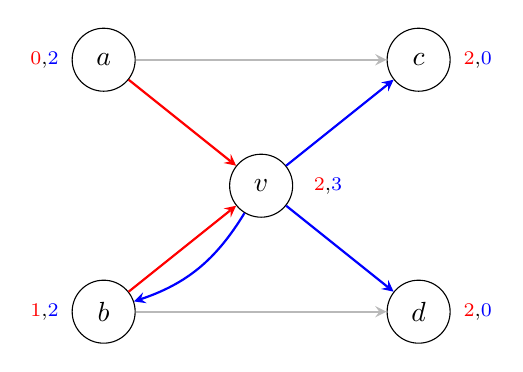
\begin{tikzpicture}[
  vtx/.style={circle, draw, minimum size=8mm},
  e/.style={->, thick, >=stealth},
  inE/.style={e, red},
  outE/.style={e, blue},
  otherE/.style={e, gray!55},
  deg/.style={font=\scriptsize, fill=white, inner sep=1pt}
]

% --- vertices ---
\node[vtx] (a) at (0, 1.6) {$a$};
\node[vtx] (b) at (0,-1.6) {$b$};
\node[vtx] (v) at (2, 0.0) {$v$};
\node[vtx] (c) at (4, 1.6) {$c$};
\node[vtx] (d) at (4,-1.6) {$d$};

% --- edges ---
% incoming to v (red)
\draw[inE] (a) -- (v);
\draw[inE] (b) -- (v);

% outgoing from v (blue)
\draw[outE] (v) -- (c);
\draw[outE] (v) -- (d);
\draw[outE] (v) to[bend left=20] (b);

% other edges (gray) for context
\draw[otherE] (a) -- (c);
\draw[otherE] (b) -- (d);

% --- (in-degree, out-degree) labels next to each vertex ---
% format: (red in-degree, blue out-degree)
\node[deg] at (-0.75, 1.6) {\textcolor{red}{0},\textcolor{blue}{2}}; % a: out to v and c
\node[deg] at (-0.75,-1.6) {\textcolor{red}{1},\textcolor{blue}{2}}; % b: in from v; out to v and d
\node[deg] at ( 2.85, 0.0) {\textcolor{red}{2},\textcolor{blue}{3}}; % v: in from a,b; out to c,d,b
\node[deg] at ( 4.75, 1.6) {\textcolor{red}{2},\textcolor{blue}{0}}; % c: in from v and a
\node[deg] at ( 4.75,-1.6) {\textcolor{red}{2},\textcolor{blue}{0}}; % d: in from v and b

\end{tikzpicture}
\caption{A directed graph where each vertex is annotated with its \textcolor{red}{in-degree} and \textcolor{blue}{out-degree} as an ordered pair \((d^{-},d^{+})\). Incoming edges are shown in \textcolor{red}{red} and outgoing edges in \textcolor{blue}{blue}.}
\label{fig:in-out-degree-pairs}
\end{figure}
